$
\begin{array}{cccc}
    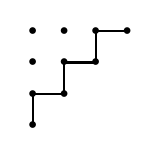
\begin{tikzpicture}[scale=.4, baseline=.5cm]
    	\draw [thick] (0,0)--(0,1); 
    	\draw [thick] (0,1)--(1,1); 
    	\draw [thick] (1,1)--(1,2); 
    	\draw [thick] (1,2)--(2,2); 
    	\draw [thick] (2,2)--(2,3); 
    	\draw [thick] (2,3)--(3,3); 
 		\foreach \x in {0, ..., 3}
    		\foreach \y in {\x, ..., 3}
    			\node (\x,\y) at (\x,\y) [inner sep=0pt] {$\scriptscriptstyle \bullet$};
    \end{tikzpicture} 
    &
    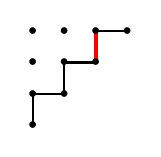
\begin{tikzpicture}[scale=.4, baseline=.5cm]
    	\draw [thick] (0,0)--(0,1); 
    	\draw [thick] (0,1)--(1,1); 
    	\draw [thick] (1,1)--(1,2); 
    	\draw [thick] (1,2)--(2,2); 
    	\draw [ultra thick, color=red] (2,2)--(2,3); 
    	\draw [thick] (2,3)--(3,3); 
 		\foreach \x in {0, ..., 3}
    		\foreach \y in {\x, ..., 3}
    			\node (\x,\y) at (\x,\y) [inner sep=0pt] {$\scriptscriptstyle \bullet$};
    \end{tikzpicture} 
    &
    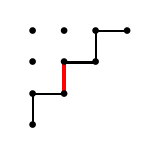
\begin{tikzpicture}[scale=.4, baseline=.5cm]
    	\draw [thick] (0,0)--(0,1); 
    	\draw [thick] (0,1)--(1,1); 
    	\draw [ultra thick, color=red] (1,1)--(1,2); 
    	\draw [thick] (1,2)--(2,2); 
    	\draw [thick] (2,2)--(2,3); 
    	\draw [thick] (2,3)--(3,3); 
 		\foreach \x in {0, ..., 3}
    		\foreach \y in {\x, ..., 3}
    			\node (\x,\y) at (\x,\y) [inner sep=0pt] {$\scriptscriptstyle \bullet$};
    \end{tikzpicture} 
    &
    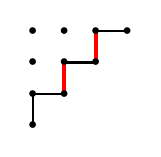
\begin{tikzpicture}[scale=.4, baseline=.5cm]
    	\draw [thick] (0,0)--(0,1); 
    	\draw [thick] (0,1)--(1,1); 
    	\draw [ultra thick, color=red] (1,1)--(1,2); 
    	\draw [thick] (1,2)--(2,2); 
    	\draw [ultra thick, color=red] (2,2)--(2,3); 
    	\draw [thick] (2,3)--(3,3); 
 		\foreach \x in {0, ..., 3}
    		\foreach \y in {\x, ..., 3}
    			\node (\x,\y) at (\x,\y) [inner sep=0pt] {$\scriptscriptstyle \bullet$};
    \end{tikzpicture} 
    \\[.8cm]
    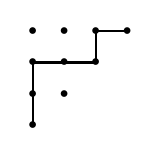
\begin{tikzpicture}[scale=.4, baseline=.5cm]
    	\draw [thick] (0,0)--(0,1); 
    	\draw [thick] (0,1)--(0,2); 
    	\draw [thick] (0,2)--(1,2); 
    	\draw [thick] (1,2)--(2,2); 
    	\draw [thick] (2,2)--(2,3); 
    	\draw [thick] (2,3)--(3,3); 
 		\foreach \x in {0, ..., 3}
    		\foreach \y in {\x, ..., 3}
    			\node (\x,\y) at (\x,\y) [inner sep=0pt] {$\scriptscriptstyle \bullet$};
    \end{tikzpicture} 
    &
    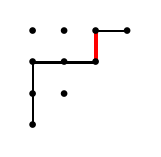
\begin{tikzpicture}[scale=.4, baseline=.5cm]
    	\draw [thick] (0,0)--(0,1); 
    	\draw [thick] (0,1)--(0,2); 
    	\draw [thick] (0,2)--(1,2); 
    	\draw [thick] (1,2)--(2,2); 
    	\draw [ultra thick, color=red] (2,2)--(2,3); 
    	\draw [thick] (2,3)--(3,3); 
 		\foreach \x in {0, ..., 3}
    		\foreach \y in {\x, ..., 3}
    			\node (\x,\y) at (\x,\y) [inner sep=0pt] {$\scriptscriptstyle \bullet$};
    \end{tikzpicture} 
    &
    &
    \\[.8cm]
    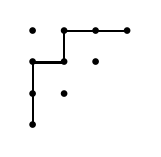
\begin{tikzpicture}[scale=.4, baseline=.5cm]
    	\draw [thick] (0,0)--(0,1); 
    	\draw [thick] (0,1)--(0,2); 
    	\draw [thick] (0,2)--(1,2); 
    	\draw [thick] (1,2)--(1,3); 
    	\draw [thick] (1,3)--(2,3); 
    	\draw [thick] (2,3)--(3,3); 
 		\foreach \x in {0, ..., 3}
    		\foreach \y in {\x, ..., 3}
    			\node (\x,\y) at (\x,\y) [inner sep=0pt] {$\scriptscriptstyle \bullet$};
    \end{tikzpicture} 
    &
    &
    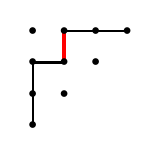
\begin{tikzpicture}[scale=.4, baseline=.5cm]
    	\draw [thick] (0,0)--(0,1); 
    	\draw [thick] (0,1)--(0,2); 
    	\draw [thick] (0,2)--(1,2); 
    	\draw [ultra thick, color=red] (1,2)--(1,3); 
    	\draw [thick] (1,3)--(2,3); 
    	\draw [thick] (2,3)--(3,3); 
 		\foreach \x in {0, ..., 3}
    		\foreach \y in {\x, ..., 3}
    			\node (\x,\y) at (\x,\y) [inner sep=0pt] {$\scriptscriptstyle \bullet$};
    \end{tikzpicture} 
    &
    \\[.8cm]
    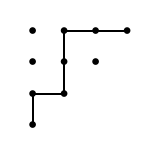
\begin{tikzpicture}[scale=.4, baseline=.5cm]
    	\draw [thick] (0,0)--(0,1); 
    	\draw [thick] (0,1)--(1,1); 
    	\draw [thick] (1,1)--(1,2); 
    	\draw [thick] (1,2)--(1,3); 
    	\draw [thick] (1,3)--(2,3); 
    	\draw [thick] (2,3)--(3,3); 
 		\foreach \x in {0, ..., 3}
    		\foreach \y in {\x, ..., 3}
    			\node (\x,\y) at (\x,\y) [inner sep=0pt] {$\scriptscriptstyle \bullet$};
    \end{tikzpicture} 
    &
    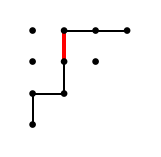
\begin{tikzpicture}[scale=.4, baseline=.5cm]
    	\draw [thick] (0,0)--(0,1); 
    	\draw [thick] (0,1)--(1,1); 
    	\draw [thick] (1,1)--(1,2); 
    	\draw [ultra thick, color=red] (1,2)--(1,3); 
    	\draw [thick] (1,3)--(2,3); 
    	\draw [thick] (2,3)--(3,3); 
 		\foreach \x in {0, ..., 3}
    		\foreach \y in {\x, ..., 3}
    			\node (\x,\y) at (\x,\y) [inner sep=0pt] {$\scriptscriptstyle \bullet$};
    \end{tikzpicture} 
    &
    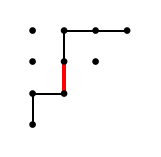
\begin{tikzpicture}[scale=.4, baseline=.5cm]
    	\draw [thick] (0,0)--(0,1); 
    	\draw [thick] (0,1)--(1,1); 
    	\draw [ultra thick, color=red] (1,1)--(1,2); 
    	\draw [thick] (1,2)--(1,3); 
    	\draw [thick] (1,3)--(2,3); 
    	\draw [thick] (2,3)--(3,3); 
 		\foreach \x in {0, ..., 3}
    		\foreach \y in {\x, ..., 3}
    			\node (\x,\y) at (\x,\y) [inner sep=0pt] {$\scriptscriptstyle \bullet$};
    \end{tikzpicture} 
    &
    \\[.8cm]
    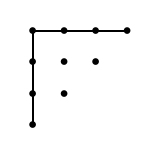
\begin{tikzpicture}[scale=.4, baseline=.5cm]
    	\draw [thick] (0,0)--(0,1); 
    	\draw [thick] (0,1)--(0,2); 
    	\draw [thick] (0,2)--(0,3); 
    	\draw [thick] (0,3)--(1,3); 
    	\draw [thick] (1,3)--(2,3); 
    	\draw [thick] (2,3)--(3,3); 
 		\foreach \x in {0, ..., 3}
    		\foreach \y in {\x, ..., 3}
    			\node (\x,\y) at (\x,\y) [inner sep=0pt] {$\scriptscriptstyle \bullet$};
    \end{tikzpicture} 
\end{array}
$